\documentclass[10pt]{beamer}
% version imprimable pour assistance
%\documentclass[10pt, green, handout]{beamer}
\usepackage[T1]{fontenc}
\usepackage[utf8]{inputenc}
\usepackage[french]{babel} % le document est en français
\usepackage{textcomp}
\usepackage{csquotes}
\usepackage{amsmath}
\usepackage{amssymb}
\usepackage{graphicx}       % pour insérer des figures
\usepackage{xcolor}         % pour définir plus de couleurs
\usepackage{tikz}
\usetikzlibrary{calc,positioning,arrows,decorations.text,decorations.pathmorphing,decorations.pathreplacing,shapes.misc}
\usepackage[absolute,overlay]{textpos}
\useinnertheme[shadow=true]{rounded}
%\setbeamercolor{block title}{bg=blue}
\usetheme{Berlin}  %Applique le theme INRA (ce dernier doit être present dans le repertoire courant)
%-------------------------------------------------------------------------------
% Quelques options pdf
%-------------------------------------------------------------------------------
\hypersetup{
pdfpagemode = FullScreen, % afficher le pdf en plein écran
pdfauthor   = {Sébastien Guyader},%
pdftitle    = {Retour sur l'école chercheurs MEXICO "Analyse de sensibilité globale, métamodélisation et optimisation de modèles complexes"},%
pdfsubject  = {Analyse de sensibilité globale, métamodélisation et optimisation de modèles complexes},%
pdfkeywords = {Analyse de sensibilité globale, optimisation, métamodélisation},%
pdfcreator  = {TeXstudio},%
pdfproducer = {INRA}%
}

%-------------------------------------------------------------------------------
\title{Retour sur l'école chercheurs MEXICO \enquote{Analyse de sensibilité globale, métamodélisation et optimisation de modèles complexes}}
\author{Sébastien Guyader}



%-------------------------------------------------------------------------------
\begin{document}

%-Title slide------------------------------------------------------------------------------
\begin{frame}
  \titlepage
\end{frame}

\section{MEXICO}

%-Slide 01------------------------------------------------------------------------
\begin{frame}{}

\begin{figure}
	\centering
	
\includegraphics[width=0.3\linewidth]{figures/logo_MEXICO}
\end{figure}

\begin{itemize}
	\item Réseau méthodologique sur les\\
	\enquote{\textcolor{red}{M}éthodes d'\textcolor{red}{EX}ploration \textcolor{red}{I}nformatique de modèles \textcolor{red}{CO}mplexes}
	\item Animé par des chercheurs du département MIA de l'INRA
	\item Autres organismes participants : IFREMER, IRSTEA, CIRAD, Université du Littoral Côte d'Opale...
	\item Objectifs :
	\begin{itemize}
		\item ouvrir les biologistes-modélisateurs au traitement stat. des simulations et à l'exploration raisonnée des modèles
		\item initier de nouveaux fronts de recherches en statistique
		\item contribuer à la réflexion méthodologique en modélisation
		\item rendre ces méthodes accessibles au modélisateur		
	\end{itemize} 
\end{itemize} 

\end{frame}

%-Slide 02------------------------------------------------------------------------
\begin{frame}{}

\begin{figure}
	\centering
	
\includegraphics[width=0.3\linewidth]{figures/logo_MEXICO}
	\label{fig:logomexico}
\end{figure}

Les actions du réseau sont organisées autour de 4 axes :

\begin{itemize}
	\item Journées thématiques : journées plus ou moins ouvertes, sur un thème méthodologique spécifique
	\item Rencontres Mexico : journées destinées aux retours d'expérience des utilisateurs des méthodes d'analyse et d'exploration de modèles
	\item Écoles-chercheurs : session de formation sur l'exploration et l'analyse de sensibilité de modèles
	\item Développements informatiques : développement d'une boîte à outils mettant ces méthodes à disposition d'utilisateurs de R ou de gestionnaires de plateformes de modélisation est en cours.
\end{itemize}

\end{frame}

%-Slide 03------------------------------------------------------------------------
\begin{frame}{}

\begin{figure}
	\centering
	
\includegraphics[width=0.3\linewidth]{figures/logo_MEXICO}
	\label{fig:logomexico}
\end{figure}

L'école chercheurs 2018 a eu lieu à La Rochelle, du 26 au 30 mars 2018 
Au sommaire des réjouissances : exposés, cours, et TP portant sur :

\begin{enumerate}
	\item La conception de plans d'expérience
	\item L'analyse de sensibilité globale et d'incertitude
	\item La calibration et l'optimisation de modèles
	\begin{enumerate}
		\item Modélisation statistique
		\item Optimisation basée sur modèles (métamodélisation)
		\item Optimisation sans métamodèle
		\item Inférence/calibration bayésienne
	\end{enumerate}
\end{enumerate}

\end{frame}

\section{Sensibilité / Incertitude}

%-Slide 04------------------------------------------------------------------------
\begin{frame}
\frametitle{Analyse d'incertitude}

\begin{block}{Question}
	Quelle incertitude sur fonction $ \mathcal{G} (x) $, et ses sources ?
\end{block}

\begin{itemize}
	\item si on connait la distribution des paramètres $ x_{1},...,x_{k} $, et si modèle simple on peut déduire la distribution de $ \mathcal{G} (x) $
	\item mais si fonction complexe, ou si la distribution des paramètres est inconnue, on échantillonne $ N $ combinaisons des paramètres (Monte Carlo, Hypercubes latins, ...)
	\item on fait appel $ N $ fois au modèle et on décrit la variation de $ \mathcal{G} (x) $
	\item la précision dépend uniquement de $ N $, et non de la dimension $ K $ du modèle $ \mathcal{G} $
\end{itemize}


\end{frame}

%-Slide 05------------------------------------------------------------------------
\begin{frame}
\frametitle{Analyse d'incertitude}
\bigskip
\bigskip
\begin{columns}
	\column{0.5\textwidth}
		N=10
		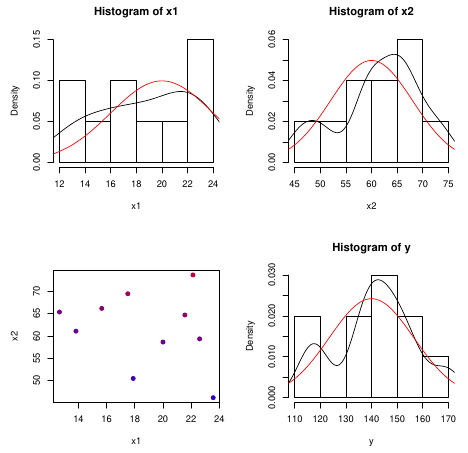
\includegraphics[width=0.9\textwidth]{figures/incertitude_1}
	\column{0.5\textwidth}
		N=1000
		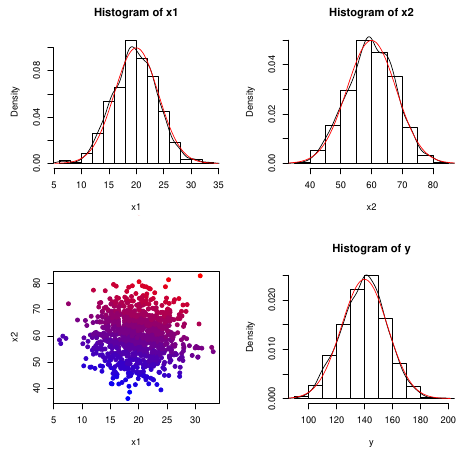
\includegraphics[width=0.9\textwidth]{figures/incertitude_2}
\end{columns}


\end{frame}

%-Slide 06------------------------------------------------------------------------
\begin{frame}

\frametitle{Analyse de sensibilité}
\bigskip
\bigskip

\begin{block}{Question}
	Quelles sont les principales sources de variation qui influencent $ \mathcal{G} (x) $ ?
	Quels paramètres sont influents ?
\end{block}

\begin{itemize}
	\item AS locale : variation de $ \mathcal{G} (x) $ autour de la valeur $ x_{0} $ (basé sur calcul de dérivées)
	\item AS globale : variation de $ \mathcal{G} (x) $ quand $ x $ varie dans son domaine d'incertitude entre $ x_{min} $ et $ x_{max} $ (basée sur calcul d'indices)
	\item on définit des indices de sensibilité, puis on les calcule en faisant varier les paramètres sur leurs domaines
\end{itemize}

\end{frame}

%-Slide 07------------------------------------------------------------------------
\begin{frame}
\frametitle{Analyse de sensibilité}

\bigskip
\bigskip

4 étapes :	
\begin{enumerate}
	\item définir les distributions des paramètres (on suppose qu'ils sont indépendants)
	\item générer des échantillons à partir de ces distributions
	\item calculer $ \mathcal{G} (x) $ pour chaque série de paramètres générée
	\item calculer les indices de sensibilité
\end{enumerate}

\end{frame}

%-Slide 07------------------------------------------------------------------------
\begin{frame}
\frametitle{Analyse de sensibilité}

\bigskip
\bigskip

2 familles de méthodes basées sur :
\begin{enumerate}
	\item criblage, discrétisation de l'espace des paramètres :
	\begin{itemize}
		\item plan factoriel/anova $ \rightarrow $ indices de sensibilité = contributions principales et totales des facteurs,\\
		$ \frac{SCE(effet principal + interaction)}{SCT} $
		\item méthode de Morris
	\end{itemize}
	\item espace des paramètres continu :
	\begin{itemize}	
		\item indices basés sur la régression
		\item indices de Sobol' estimés par échantillonnage intensif
		\item Pick \& Freeze, et extended FAST
	\end{itemize}
\end{enumerate}

\end{frame}

%-Slide 07------------------------------------------------------------------------
\begin{frame}
\frametitle{Analyse de sensibilité}

\bigskip
\bigskip

Criblage (1)
\bigskip

L'ANOVA nécessite un plan factoriel pour décompostion totale de la variance
	\begin{itemize}
		\item un plan factoriel complet est très grand (chaque facteur est décomposé en niveaux, et tous les niveaux sont croisés)
		\item ex : un modèle à 20 paramètres incertains, avec 3 niveaux il faut $ 3^{20} = 3 486 784 401 $ évaluations du modèle
		\item si 1 évaluation prend 0.01 seconde, il faut 24.2 jours (24.2 * 200 Watts = 116 226 kWh, coût d'environ 11.6 k€ à 10cts / kWh) = consommation annuelle de 16 foyers français
		\item les plans fractionnaires sont utiles
	\end{itemize}



\end{frame}

%-Slide 08------------------------------------------------------------------------
\begin{frame}
\frametitle{Analyse de sensibilité}

\bigskip


Criblage (1)
\bigskip
\\
Plan factoriel : 3 facteurs (paramètres), 5 niveaux
\centering
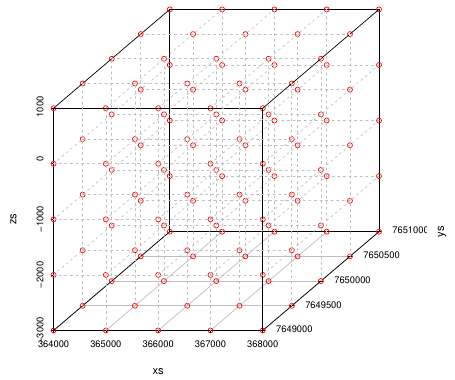
\includegraphics[width=0.6\textwidth]{figures/plan_factoriel}


\end{frame}

%-Slide 09------------------------------------------------------------------------
\begin{frame}
\frametitle{Analyse de sensibilité}

\bigskip
\bigskip

Criblage (2)
\bigskip

\begin{itemize}
	\item Morris : exploration "astucienne" de l'espace des paramètres
	\begin{enumerate}	
		\item discrétiser l'espace $ \rightarrow $ point de départ aléatoire $ \rightarrow $ déplacement sur 1 seul facteur à la fois (OAT) $ \Rightarrow $ 1 trajectoire $ K $ déplacements ($ K+1 $ points)
		\item mesurer l'importance du facteur $ x_{i} $ sur chaque trajectoire n évaluant le modèle en fonction de la taille du saut
		\begin{itemize}
			\item effet élémentaire (effet d'un saut rapporté à la taille du saut)
			\item effet moyen (somme effets des trajectoires divisé par le nb de trajectoires)
			\item effet absolu moyen (prend la valeur absolue des effets élémentaires)
			\item écart-type des effets élémentaires
		\end{itemize}
	\end{enumerate}
\end{itemize}

\end{frame}

%-Slide 10------------------------------------------------------------------------
\begin{frame}
\frametitle{Analyse de sensibilité}

\bigskip
\bigskip

Criblage (2)
\bigskip
\\

\centering
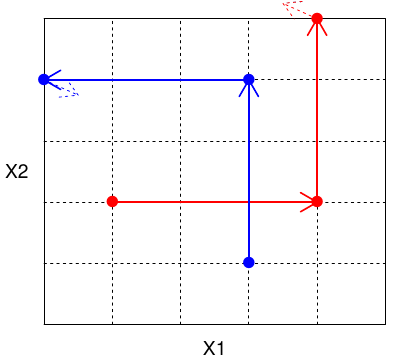
\includegraphics[width=0.4\textwidth]{figures/Morris}

\end{frame}

%-Slide 11------------------------------------------------------------------------
\begin{frame}
\frametitle{Analyse de sensibilité}

\bigskip
\bigskip

Criblage (2)
\bigskip
\\

\centering
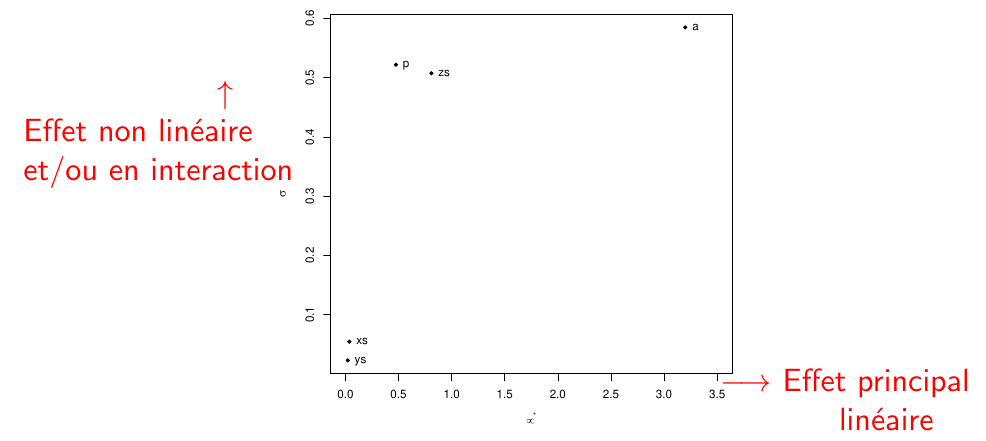
\includegraphics[width=1\textwidth]{figures/Res_Morris}

\end{frame}

%-Slide 12------------------------------------------------------------------------
\begin{frame}
\frametitle{Analyse de sensibilité}

\bigskip
\bigskip

Espace continu des paramètres (1)


\begin{itemize}
	\item tirer les entrées $ X $ sur leur intervalle (hypercube latin, Monte Carlo, ou suite à faible discrépance)
	\item 2 méthodes :
	\begin{enumerate}	
		\item indices basés sur la régression : coefficient de corrélation linéaire ("src") ou partielle ("pcc", plus approprié s'il y a corrélation entre les facteurs)
		\item décomposition d'Hoeffding - Sobol' : décomposition analogue à celle de la variance, indices de sensibilité = effets principal des paramètres et de leur interaction
	\end{enumerate}
\end{itemize}
\begin{itemize}
	\item problème : ces méthodes nécessitent de nombreux appels au code
	\item il y a des méthodes alternatives pour estimer les indices :
	\begin{itemize}
		\item méthode Sobol' - Saltelli ou Pick \& Freeze
		\item méthode FAST (Fourier Amplitude Sensitivity Test)
		\item passage par un métamodèle
	\end{itemize}
\end{itemize}

\end{frame}

%-Slide 13------------------------------------------------------------------------
\begin{frame}
\frametitle{Analyse de sensibilité}

\bigskip
\bigskip

Espace continu des paramètres (2)
\bigskip

\begin{itemize}
	\item méthode Sobol' ou Pick \& Freeze
	\begin{itemize}
		\item 2 échantillonnages A et B (hypercube latin, Monte Carlo, ou suite à faible discrépance), taille $ N*K $
		\item évaluations sur $ N*(K+2) $ combinaisons C issues de A et B
		\item estimation des indices
		\item évaluation de la précision par répétition ou bootstrap
	\end{itemize}
	\item méthode FAST
	\begin{itemize}
	\item échantillonnage par trajectoire déterministe remplissant l'espace ("space-filling path")
	\item choix raisonné du jeu de fréquences $ \omega_{i} $ (harmoniques distinctes entre facteurs jusqu'à l'ordre M (4 à 6)
	\item estimation par analyse fréquentielle
	\item eFAST (FAST étendu) : 1 trajectoire FAST par paramètre $ x_{i} $
	\end{itemize}	
\end{itemize}

\end{frame}

%-Slide 14------------------------------------------------------------------------
\begin{frame}
\frametitle{Analyse de sensibilité}

\bigskip
\bigskip

Criblage (2)
\bigskip
\\
Sobol

\centering
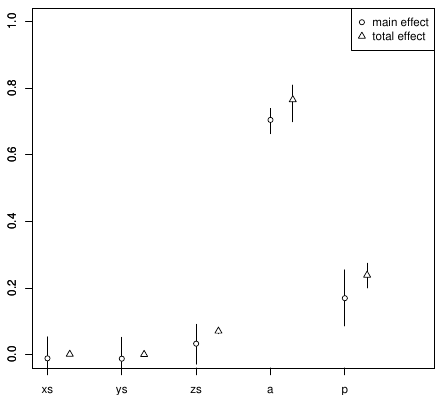
\includegraphics[width=0.5\textwidth]{figures/sobol}

\end{frame}

%-Slide 15------------------------------------------------------------------------
\begin{frame}
\frametitle{Analyse de sensibilité}

\bigskip
\bigskip

Criblage (2)
\bigskip
\\
Fast

\centering
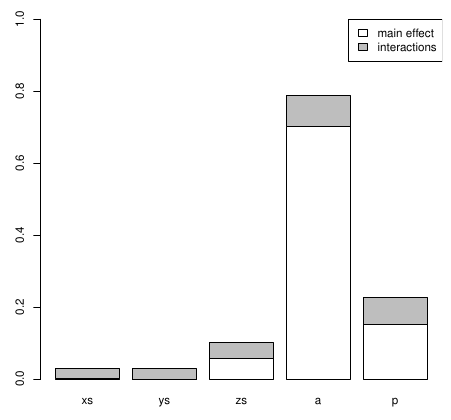
\includegraphics[width=0.5\textwidth]{figures/fast99}

\end{frame}

\section{Plans d'expérience}

%-Slide 13------------------------------------------------------------------------
\begin{frame}

\begin{itemize}
\item Souvent, on approche le vrai modèle à l'aide d'une fonction mathématique
\item Il faut évaluer la fonction de nombreuses fois, question : pour un budget de $ n $ appels à la fonction, quels points de l'espace des paramètres doit-on évaluer ?
\item Il faut une stratégie pour choisir les points à évaluer :
\begin{itemize}
	\item "One at a Time" (OAT)
	\item Pans factoriels
	\item Stratégies de remplissage de l'espace
\end{itemize}
\end{itemize}

\end{frame}

%-Slide 14------------------------------------------------------------------------
\begin{frame}
\frametitle{OAT}
\bigskip

\begin{itemize}
	\item Toutes les variables sont fixées, sauf 1 qui varie pour évaluer son influence sur G(x)
	\item Il faut plus de 2 niveaux pour estimer les effets quadratiques
\end{itemize}

\begin{columns}
	\column{0.5\textwidth}
	2 niveaux
	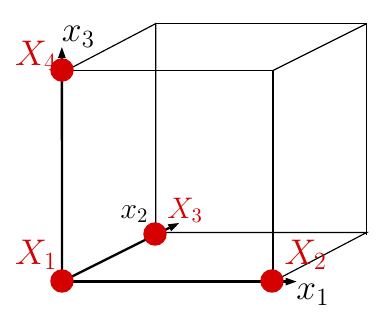
\includegraphics[width=0.9\textwidth]{figures/OAT_1}
	\column{0.5\textwidth}
	3 niveaux
	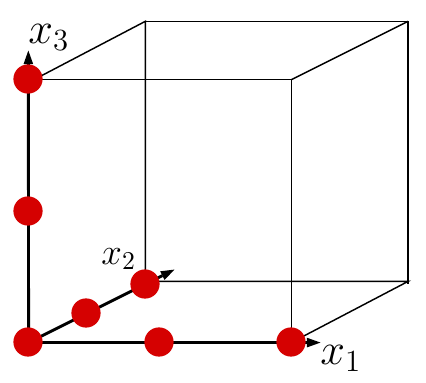
\includegraphics[width=0.8\textwidth]{figures/OAT_2}
\end{columns}

\end{frame}

%-Slide 15------------------------------------------------------------------------
\begin{frame}
\frametitle{Plans factoriels}
\bigskip

\begin{itemize}
	\item Toutes les combinaisons de paramètres sont testées
	\item Le plus simple à 2 niveaux (min et max), on peut tester plus de niveaux
	\item Problème : le temps de calcul explose avec le nombre de paramètres et de niveaux
\end{itemize}

\begin{columns}
	\column{0.5\textwidth}
	2 niveaux
	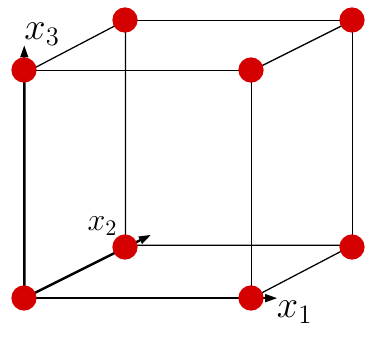
\includegraphics[width=0.8\textwidth]{figures/plan_factoriel_1}
	\column{0.5\textwidth}
	3 niveaux
	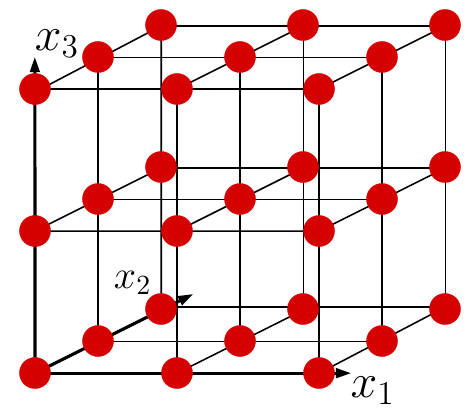
\includegraphics[width=0.8\textwidth]{figures/plan_factoriel_2}
\end{columns}

\end{frame}

%-Slide 16------------------------------------------------------------------------
\begin{frame}
\frametitle{Stratégies de remplissage de l'espace}
\bigskip

\begin{itemize}
	\item Quels critères pour évaluer le remplissage de l'espace :
	\begin{itemize}
		\item "maximin" (maximiser la distance minimale entre 2 points) et "minimax" (minimiser la distance maximale entre 2 points)
		\item "discrépance" : compare le nb de points dans un hyper-rectangle au nb de points attendus par distrib uniforme
	\end{itemize}
	\item Il y a 3 principales stratégies de remplissage :
	\begin{itemize}
		\item Hypercubes latins
		\item Séquences à faible discrépance
		\item Tesselation centroïde de Voronoi
	\end{itemize}
\end{itemize}

\end{frame}

%-Slide 17------------------------------------------------------------------------
\begin{frame}
\frametitle{Hypercubes latins (lhs)}
\bigskip

\begin{itemize}
	\item découpage du domaine en $ n^{d} $ blocs avec seulement 1 point par "ligne" et "colonne"
	\item à combiner avec critère tel que "maximin"
	\begin{center}
		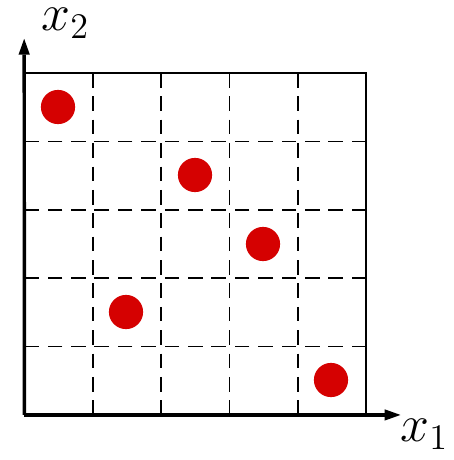
\includegraphics[width=0.4\textwidth]{figures/lhs}
	\end{center}
	\item optimisation d'un LHS par méthode de "Morris \& Mitchell"
\end{itemize}

\end{frame}

%-Slide 17------------------------------------------------------------------------
\begin{frame}
\frametitle{Séries à faible discrépance}
\bigskip

\begin{itemize}
	\item séquences déterministes qui convergent vers une distribution uniforme
	\begin{center}
		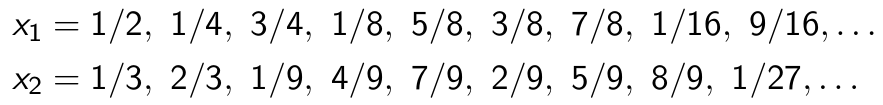
\includegraphics[width=0.6\textwidth]{figures/seq_halton1}
	\end{center}
	\item couvrent l'espace rapidement et de manière homogène
	\begin{center}
		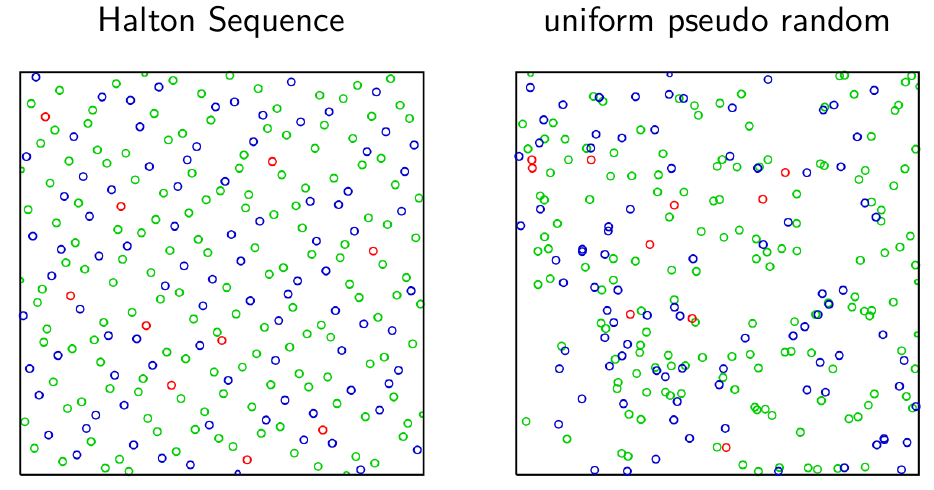
\includegraphics[width=0.7\textwidth]{figures/seq_halton}
	\end{center}
\end{itemize}

\end{frame}

%-Slide 18------------------------------------------------------------------------
\begin{frame}
\frametitle{Tesselation centroïde de Voronoi}
\bigskip

\begin{itemize}
	\item partition de l'espace en cellules à partir d'un jeu de points, telle que chaque point d'une cellule est plus proche de son "germe" que de tout autre point de l'espace ("zone d'influence")
	\item algorithme de Lloyd pour la tesselation centroïde
	\begin{center}
		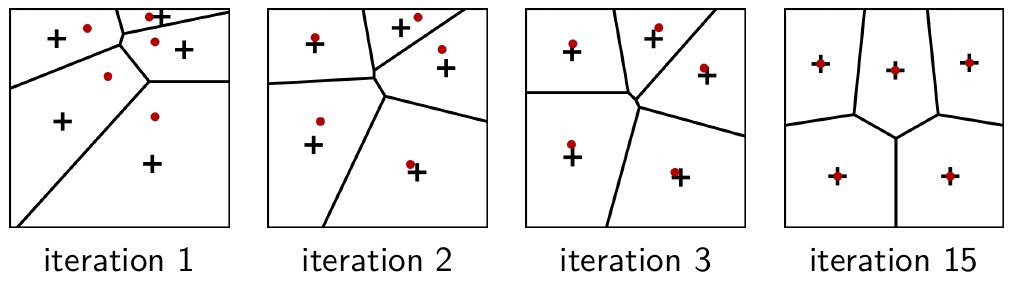
\includegraphics[width=0.9\textwidth]{figures/voronoi}
	\end{center}
	\item autre algorithme : k-means
\end{itemize}

\end{frame}

\section{Calibration / optimisation}

%-Slide 19------------------------------------------------------------------------
\begin{frame}

\begin{block}{Calibration}
	Processus d'ajustement des paramètres d'un modèle en intégrant l'incertitude des paramètres et/ou du modèle, pour obtenir une représentation du système modélisé qui satisfasse un critère prédéfini
\end{block}
\bigskip
Pour des modèles simples, la résolution analytique du problème est possible, mais pas pour des modèles complexes (nombreux paramètres, nombreuses sorties, processus mal connus)

\end{frame}

%-Slide 20------------------------------------------------------------------------
\begin{frame}

Calibrer pour :
\begin{itemize}
	\item estimer les paramètres pas ou difficilement mesurables
	\item comprendre le fonctionnement du système étudié
	\item crédibiliser/améliorer le modèle pour l'utiliser en décision, prédiction...
\end{itemize}
\bigskip
Objectif de la calibration :\\
 trouver les valeurs optimales des paramètres qui minimisent la différence entre $ Y_{obs} $ et $ Y_{sim} $
\bigskip

C'est donc l'optimisation d'une fonction mathématique (fonction d'objectif), avec 3 cas :
\begin{itemize}
	\item pas d'hypothèse de distrib. sur $ Y $ ni sur $ X $ $ \rightarrow $ analyse numérique ou statistique inférentielle
	\item hypothèse de distrib. sur $ Y $, mais pas sur $ X $ $ \rightarrow $ statistique inférentielle
	\item hypothèses de distrib sur $ Y $ et sur $ X $ $ \rightarrow $ statistique bayésienne
\end{itemize}

\end{frame}

%-Slide 21------------------------------------------------------------------------
\begin{frame}
Commencer par construire une première fonction d'objectif :
\begin{itemize}
	\item les plus communes : moindres carrés, vraisemblance
	\item plus spécifiques : ABC (Approximate Bayesian Computation)
	\item optimisation multi-objectifs : pondérations, fronts de Pareto
\end{itemize}
\bigskip

Évaluer la qualité de l'optimisation :
\begin{itemize}
	\item convergence, global/local (est-on dans tombé un creux ?)
	\item identifiabilité des paramètres (est-ce que plusieurs solutions donnent un même optimum ?)
\end{itemize}
\bigskip

A chaque itération, calcul d'un ensemble de solutions et des valeurs de la fonction d'objectif associée  : trace de l'algorithme dans l'espace $ Y $ et l'espace $ X $

\end{frame}

%-Slide 22------------------------------------------------------------------------
\begin{frame}
\frametitle{Modélisation statistique}

Les modèles statistiques sont utilisés pour :

\begin{itemize}
	\item interpoler ou approximer des fonctions
	\item calculer des quantités d'intérêt (valeur moyenne, optimum, minimum...)
	\item mesurer l'erreur
\end{itemize}
\bigskip

Il y 2 principaux types de modèles statistiques :
\begin{itemize}
	\item régression linéaire
	\item régression de processus gaussiens
\end{itemize}

\end{frame}

%-Slide 23------------------------------------------------------------------------
\begin{frame}
\frametitle{Processus gaussiens}

\begin{itemize}
	\item Basé sur la distribution Normale de $ X $ (jeu de points d'observation)
	\item Propriété : une combinaison linéaire de variables aléatoires indépendantes suit toujours une loi Normale
	\item la distribution Gaussienne multivariée peut être généralisée par un processus aléatoire, caractérisé par ses fonctions de moyenne et de covariance (ou noyau)
	\item on peut générer des vecteurs aléatoires à l'aide fonctions de covariance connues (constante, bruit blanc, exponentiel, Matern 3/2 et 5/2, gaussien...)
\end{itemize}

\end{frame}

%-Slide 24------------------------------------------------------------------------
\begin{frame}
\frametitle{Processus gaussiens}

Régression sur processus gaussiens :
\begin{itemize}
	\item on part de l'observation de la fonction $ Y=f(X) $ sur un jeu de points X
	\item on ne connait pas $ f(X) $, mais on suppose qu'elle suit le chemin d'un processus Gaussien $ Z \sim \mathcal{N}(0, k) $
	\item on calcule analytiquement la distribution \textit{a posteriori} $ Y(\cdotp)|Y(X)=Y $ : échantillon de chemins qui passent par les points d'observation
\end{itemize}

Propriétés :
\begin{itemize}
	\item permet d'interpoler entre les points
	\item il faut choisir le noyau en fonction des \textit{a priori} sur la fonction à étudier
	\item la variance de prédiction dépend uniquement du noyau choisi
	\item la prédiction de la moyenne ne dépend pas du paramètre de variance
	\item on peut aussi ajouter du bruit (incertitude) sur les observations
\end{itemize}

\end{frame}

%-Slide 25------------------------------------------------------------------------
\begin{frame}
\frametitle{Processus gaussiens}

\centering
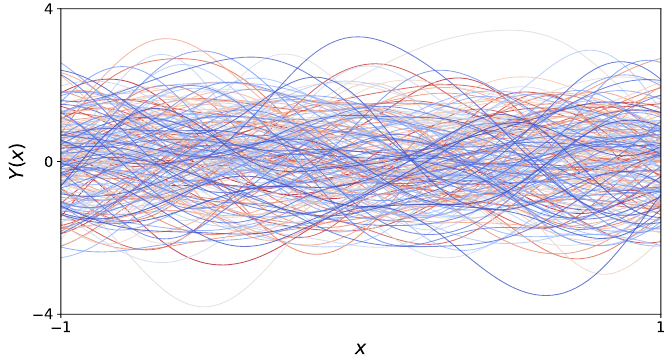
\includegraphics[width=0.9\textwidth]{figures/gaussian_1}

\end{frame}

%-Slide 26------------------------------------------------------------------------
\begin{frame}
\frametitle{Processus gaussiens}

\centering
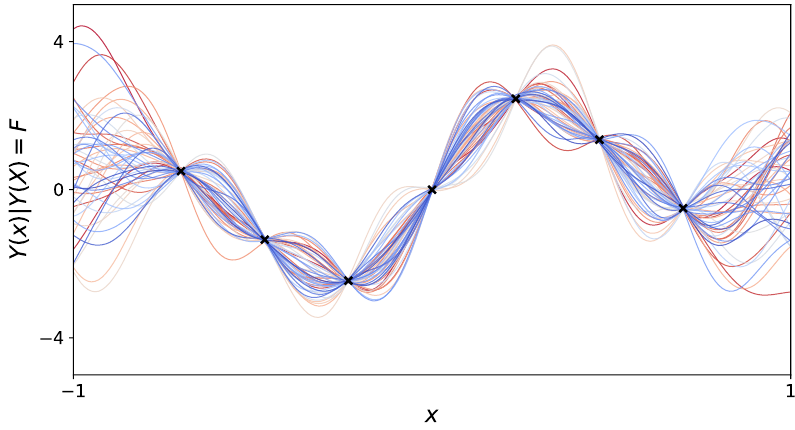
\includegraphics[width=0.9\textwidth]{figures/gaussian_2}

\end{frame}

%-Slide 27------------------------------------------------------------------------
\begin{frame}
\frametitle{Processus gaussiens}

La régression sur processus gaussiens en pratique :
\begin{enumerate}
	\item Créer un plan d'expérience (quel budget global pour l'évaluation ?)
	\item Choisir un noyau\\
	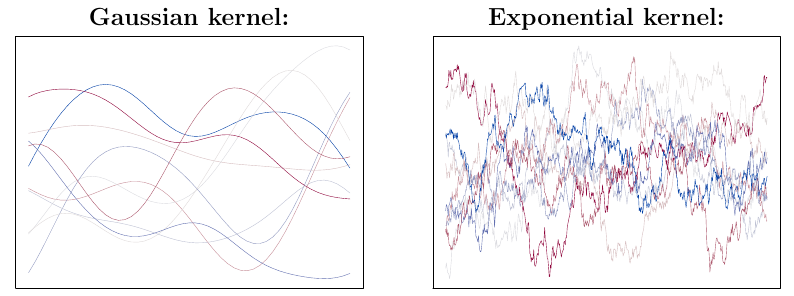
\includegraphics[width=0.7\textwidth]{figures/gaussian_3}
	\item Estimer les paramètres (max. vraisemblance, validation croisée, multiples départs)
	\item Valider le modèle (jeu de test, Leave-one-out pour moyenne et intervalles de confiance, leave-k-out pour covariances)
\end{enumerate}
Souvent, on fait plusieurs itérations des étapes 2, 3 et 4

\end{frame}

%-Slide 28------------------------------------------------------------------------
\begin{frame}
\frametitle{Optimisation basée sur métamodèles}

L'optimisation fait de nombreux appels au code, il peut être utile d'avoir recours à un métamodèle\\
\bigskip
On espère qu'à la fin, l'optimum trouvé par le métamodèle soit proche de celui du modèle réel\\
\bigskip
Compromis à trouver entre exploration/intensification\\
\bigskip
Optimisation globale :
\begin{itemize}
	\item une phase d'exploration (recherche partout dans l'espace pour ne pas rater la zone optimale)
	\item une phase d'intensification une fois la zone identifiée (on recherche le minimum local)
\end{itemize}
Remarque : il existe une méthode d'optimisation globale sans métamodèle : DIRECT (DIviding RECTangles)

\end{frame}

%-Slide 29------------------------------------------------------------------------
\begin{frame}
\frametitle{Optimisation par krigeage}

Algorithme "Efficient Global Optimization" (EGO) :
\begin{itemize}
	\item on cherche un bon compromis entre l'exploitation des bons résultats des itérations précédentes, et l'exploration pour les itérations à venir
	\item on commence par établir un plan d'expérience
	\item on calcule la fonction d'objectif $ F $ sur ces points
	\item on élabore un métamodèle, par exemple un modèle de RPG
	\item en se basant sur les intervalles de confiance et la valeur optimale actuelle de la fonction d'objectif, on calcule la valeur d' "Expected Improvement" (quelles zones sont suceptibles d'héberger l'optimum)
	\item on ajoute un point là où l'EI est plus élevé
	\item on réitère
	\item on arrête l'algorithme quand on a atteint un seuil défini d'itérations
	\item si on n'a pas trouvé d'optimum, on recommence avec un nouveau modèle RPG
\end{itemize}
Remarque : il existe une méthode d'optimisation globale sans métamodèle : DIRECT (DIviding RECTangles)

\end{frame}

%-Slide 30------------------------------------------------------------------------
\begin{frame}
\frametitle{Optimisation par krigeage}

\begin{overprint}
	\centering
	\onslide<1> Iteration 1\\ 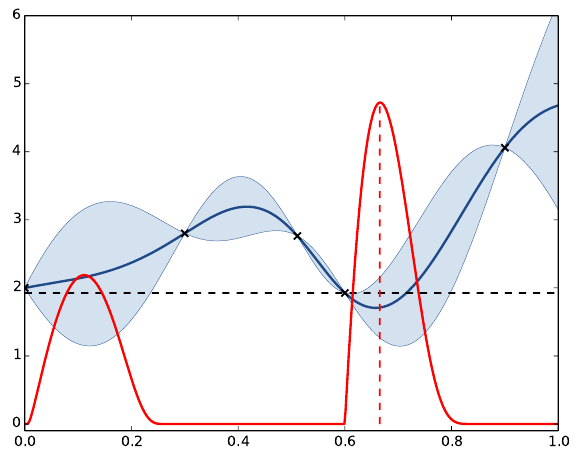
\includegraphics[width=0.7\textwidth]{figures/ego_1}
	\onslide<2> Iteration 2\\ 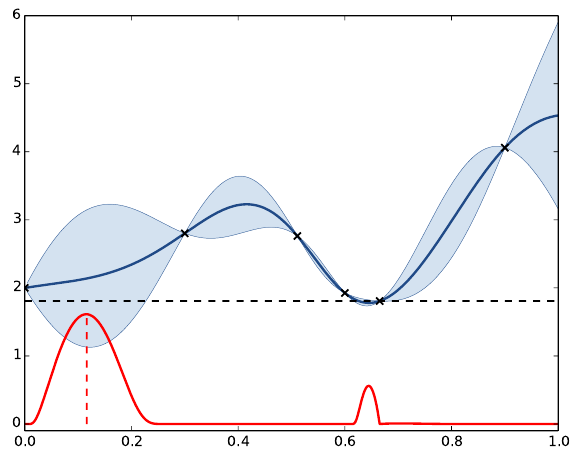
\includegraphics[width=0.7\textwidth]{figures/ego_2}
	\onslide<3> Iteration 3\\ 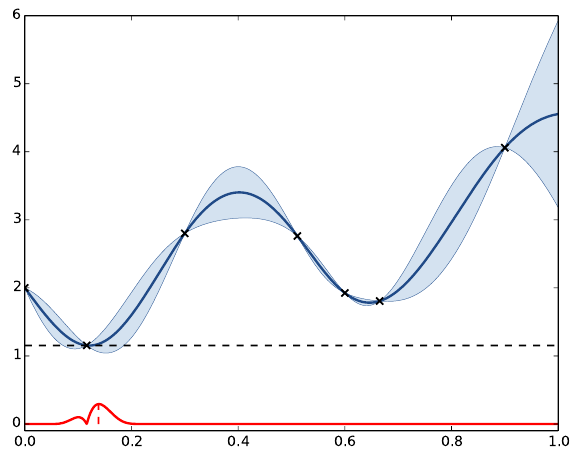
\includegraphics[width=0.7\textwidth]{figures/ego_3}
	\onslide<4> Iteration 4\\ 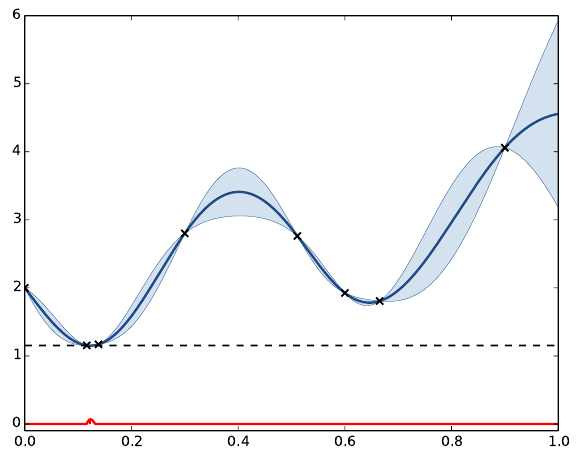
\includegraphics[width=0.7\textwidth]{figures/ego_4}
	\onslide<5> Iteration 5\\ 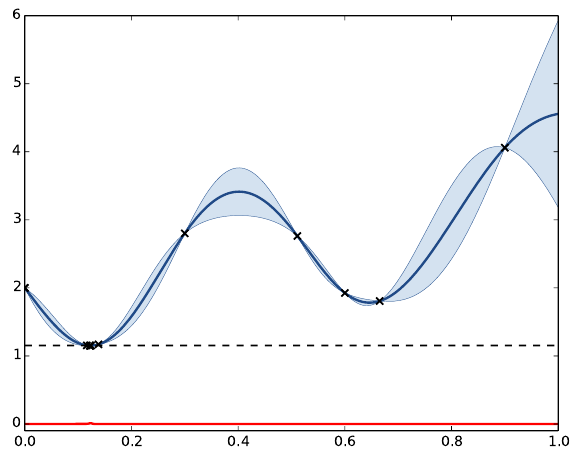
\includegraphics[width=0.7\textwidth]{figures/ego_5}
\end{overprint}

\end{frame}

%-Slide 31------------------------------------------------------------------------
\begin{frame}
\frametitle{Optimisation sans métamodèle}

Nelder-Mead :
\begin{itemize}
	\item on construit des simplex ($ d+1 $ points), on ajoute 1 point à l'opposé du point le moins bon
	\item on évalue $ F $ à ce point, si pas d'amélioration par rapport au meilleur point, stop (phase de "réflexion")
	\item si amélioration, on ajoute un point dans la même direction (on augmente la taille du pas, phase "expension")
	\item en fonction du résultat, stop ou phase de "contraction" ou de "rétractation"
\end{itemize}

\end{frame}

%-Slide 32------------------------------------------------------------------------
\begin{frame}
\frametitle{Optimisation sans métamodèle}

Nelder-Mead\\

\centering
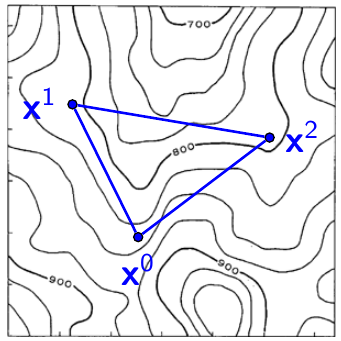
\includegraphics[width=0.3\textwidth]{figures/simplex_1}
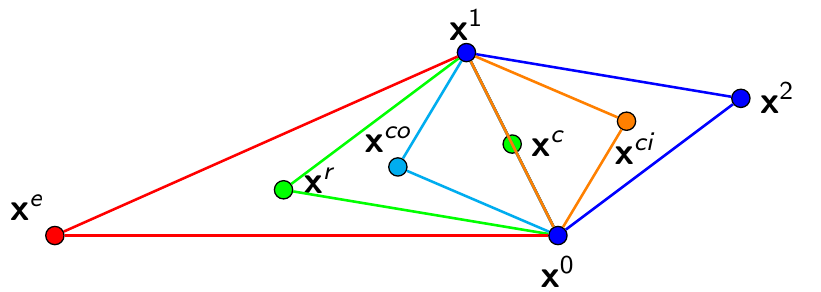
\includegraphics[width=0.7\textwidth]{figures/simplex_2}

\end{frame}

%-Slide 33------------------------------------------------------------------------
\begin{frame}
\frametitle{Optimisation sans métamodèle}

CMA-ES :
\begin{itemize}
	\item au lieu de simplex, basé sur l'échantillonnage et l'estimation d'une distribution Normale multivariée
	\item on évalue la fonction d'objectif sur un premier point
	\item on échantillonne de nouveaux points selon une distribution centrée sur le premier point
	\item on évalue la fonction à ces nouveaux points
	\item on garde les meilleurs points, on réitère en centrant la nouvelle distribution sur la moyenne des meilleurs points
	\item la direction et la taille du pas (variance) sont adaptés à chaque itération
\end{itemize}

\end{frame}

%-Slide 34------------------------------------------------------------------------
\begin{frame}
\frametitle{Optimisation sans métamodèle}

CMA-ES\\

\begin{center}
	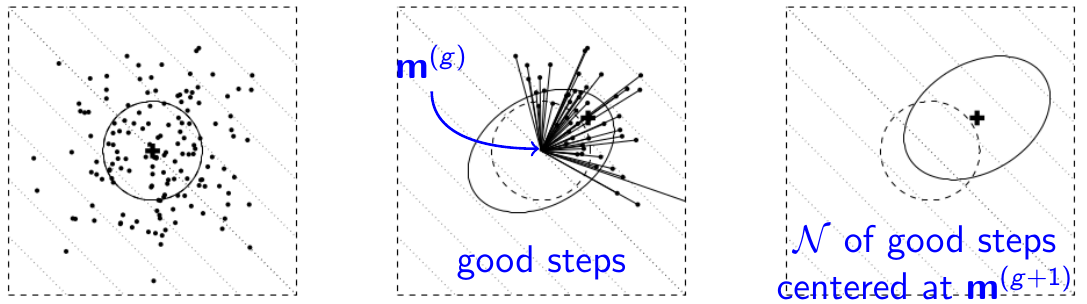
\includegraphics[width=1\textwidth]{figures/cma-es}
\end{center}

Les algorithmes Nelder-Mead et CMA-ES sont plutôt locaux et peuvent rater l'optimum global
Des variantes avec "restart" permettent de mieux explorer l'ensemble de l'espace

\end{frame}

%-Slide 35------------------------------------------------------------------------
\begin{frame}
\frametitle{Inférence/calibration bayésienne}

On considère un paramètre à estimer comme étant une variable aléatoire au même titre que les observations\\
\medskip
On cherche à caractériser la distribution \textit{a posteriori} des paramètres du modèle à l'aide de la formule de Bayes : $ [\theta|y] = \frac{[\theta][y|\theta]}{[y]} $\\
\medskip
Principe général : à partir de la connaissance \textit{a priori} de $ [\theta] $, des données $ [y|\theta] $ et de la vraisemblance, on met à jour la connaissance de $ [\theta|y] $\\
\medskip
Modèle non hiérarchique : il suffit de la vraisemblance et de l'\textit{a priori} pour estimer l'\textit{a posteriori}\\
\medskip
Modèle hiérarchique : exemple quand un paramètre varie entre individus ou sites $\rightarrow$ hyper-paramètres à estimer en plus\\
\medskip
Problème : multiples intégrales à calculer $\rightarrow$ utilisation de méthodes numériques stochastiques pour générer un échantillon issu de la distribution \textit{a posteriori}

\end{frame}

%-Slide 36------------------------------------------------------------------------
\begin{frame}
\frametitle{Inférence/calibration bayésienne}

A quoi sert l'échantillon issu de la loi \textit{a posteriori} :
\begin{itemize}
	\item connaître intimement la loi \textit{a posteriori}
	\item estimer la densité \textit{a posteriori}
	\item estimer les moments \textit{a posteriori} (espérance, variance)
	\item estimer des intervalles de crédibilité
\end{itemize}

Méthodes :
\begin{itemize}
	\item ré-échantillonnage ("sampling importance resampling")
	\item Monte Carlo par chaîne de Markov (MCMC) : génération d'une chaîne (séquence de réalisations dépendantes de $ \theta $)
	\item échantillonneur de Gibbs (loi à l'itération $ i $ repose sur une loi conditionnelle à $ i-1 $)
	\item algorithme Metropolis-Hastings (loi arbitraire au lieu de conditionnelle)
\end{itemize}

\end{frame}

%-Slide 37------------------------------------------------------------------------
\begin{frame}
\frametitle{Inférence/calibration bayésienne}

A la fin du processus, diagnostiquer la convergence des chaînes (stationnarité, variances intra- et interchaînes)\\
\medskip
Logiciels souvent utilisés : WinBUGS, OpenBUGS\\
\medskip
Problème : le calcul analytique de la vraisemblance peut devenir rapidement infaisable pour des modèles complexes\\
\medskip
Solution : méthodes Approximate Bayesian Computation (ABC), permettent de ne pas mesurer la vraisemblance\\
\medskip
Elles réalisent des simulations, et comparent les résultats avec les données observées pour construire la distribution \textit{a posteriori} à chaque itération

\end{frame}

%-Slide 38------------------------------------------------------------------------
\begin{frame}
\frametitle{Inférence/calibration bayésienne}

\begin{center}
	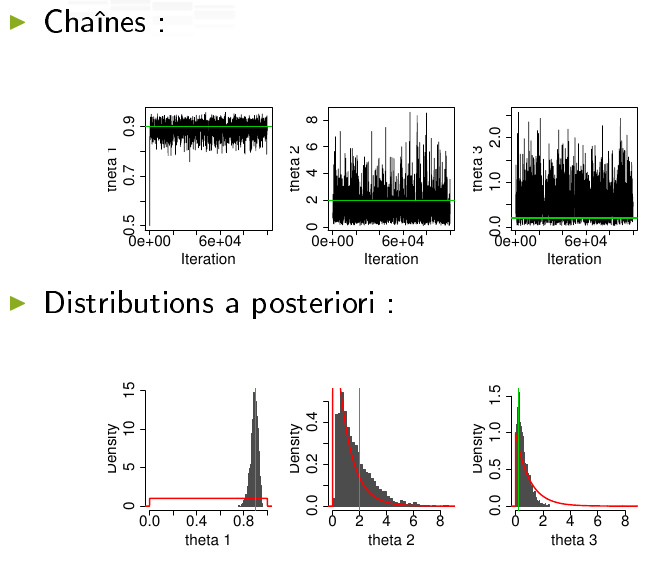
\includegraphics[width=0.75\textwidth]{figures/bayesian}
\end{center}

\end{frame}

\section{Synthèse}

%-Slide 39------------------------------------------------------------------------
\begin{frame}
\frametitle{Synthèse : méthodes d'analyse de sensibilité}

\begin{center}
	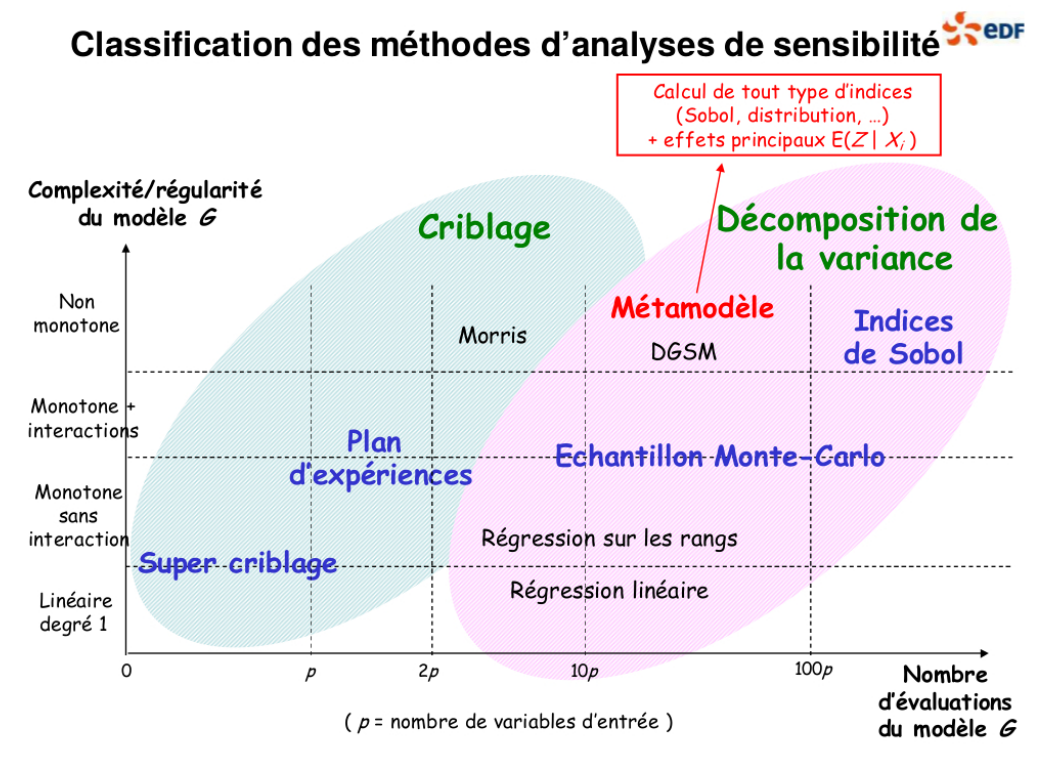
\includegraphics[width=0.9\textwidth]{figures/synthese_as}
\end{center}

\end{frame}

%-Slide 39------------------------------------------------------------------------
\begin{frame}
\frametitle{Synthèse : méthodes de calibration/optimisation/inférence}

\begin{center}
	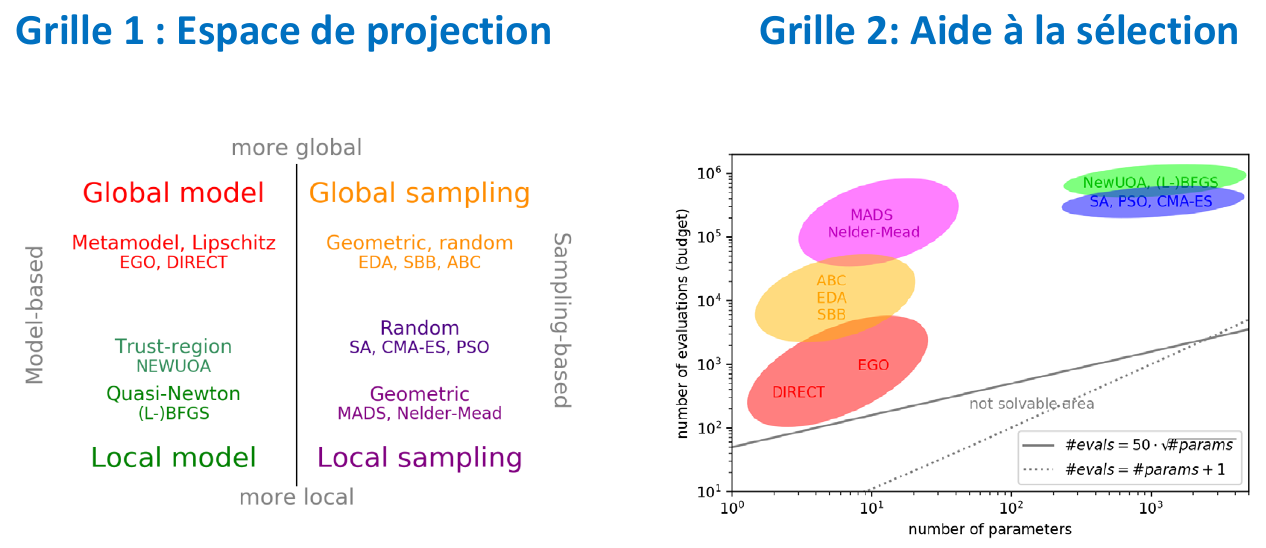
\includegraphics[width=1\textwidth]{figures/grille_calibration_1}
\end{center}

\end{frame}

%-Slide 41------------------------------------------------------------------------
\begin{frame}
\frametitle{Synthèse : implémentations dans R}

\begin{itemize}
	\item \texttt{lhs} (création de plans d'expériences par hypercubes latins)
	\item \texttt{sensitivity} (morris, sobol, src, pcc, fast)
	\item \texttt{DiceDesign} (plans d'expérience, dont hypercubes latins))
	\item \texttt{DiceEval} (construction et évaluation de métamodèles)
	\item \texttt{DiceKriging} (estimation, validation et prediction de modèles de krigeage)
	\item \texttt{DiceView} (construction de graphiques pour les métamodèles de krigeage)
	\item \texttt{DiceOptim} (optimisation par EGO, optimisation avec bruit)
	\item \texttt{cmaes} (optimisation par CMA-ES)
	\item \texttt{optim} (optimisation par Nelder-Mead)
	\item \texttt{GPareto} (optimisation multi-objectif)
	\item \texttt{R2OpenBUGS} (interagit avec OpenBUGS pour l'inférence bayésienne, avec échantillonneur de Gibs)
	\item \texttt{easyABC} (méthode ABC)
\end{itemize}

\end{frame}

\section{Modèle anthracnose}

%-Slide 42------------------------------------------------------------------------
\begin{frame}
\frametitle{Structure du modèle}

\begin{center}
	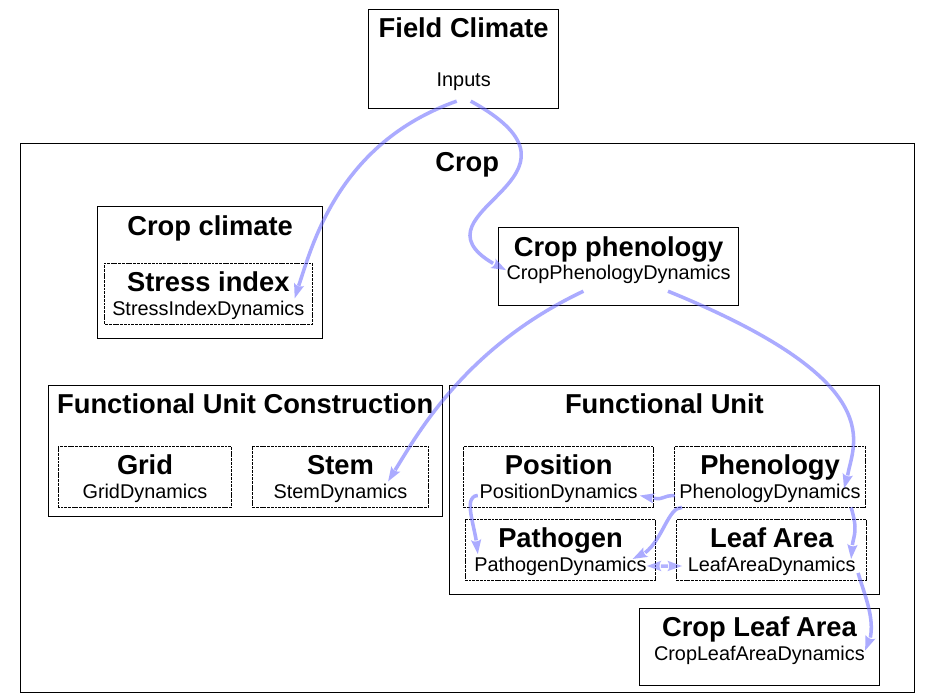
\includegraphics[width=0.8\textwidth]{figures/archidemio_formel}
\end{center}

\end{frame}

%-Slide 43------------------------------------------------------------------------
\begin{frame}
\frametitle{Dynamique des surfaces foliaires}

\begin{block}{Dynamique foliaire}	
	\begin{equation*}
	\begin{cases}
	Z(t) = \frac{Z_{max}}{1 + e^{-k_z \cdot (t-t_z)}}\\
	E(t) = \frac{E_{max}}{1 + e^{-k_e \cdot (t-t_e)}}\\
	S(t) = \frac{E_{max}}{1 + e^{-k_s \cdot (t-t_s)}}\\
	\end{cases}
	\displaystyle A(t) = E(t) - R(t)
	\end{equation*}
\end{block}

\begin{block}{Résistance ontogénique : fonction de l'âge des feuilles}	
	\begin{equation*}
	\rho(t_d) = 1 - \frac{1}{1 + e^{-k_r \cdot (t-t_r)}}
	\end{equation*}
\end{block}

\begin{block}{Porosité : fonction de la densité foliaire}	
	\begin{equation*}
	\phi_d = \phi_0 \cdot \frac{E_d - R_d}{Z_d}
	\end{equation*}
\end{block}

\end{frame}

%-Slide 44------------------------------------------------------------------------
\begin{frame}
\frametitle{Dynamique du pathogène}

\begin{block}{Dynamique des surfaces malades}	
	\begin{equation*}
	\begin{cases}
	\Delta H = \Delta E 
	- \left ( \tau_u \cdot I \cdot \frac{H}{E} \cdot \rho_d \cdot \theta_d \right )  
	- \left ( \delta i_d \cdot \frac{H}{E} \cdot \rho_d \cdot \theta_d \right )
	- \left ( \Delta S \cdot \frac{H}{A} \right )\\
	
	\Delta L = 
	\left ( \tau_u \cdot I \cdot \frac{H}{E} \cdot \rho_d \cdot \theta_d \right )   
	+ \left ( \delta i_d \cdot \frac{H}{E} \cdot \rho_d \cdot \theta_d \right )
	- \left ( \frac{1}{lp} \cdot L \right )
	- \left ( \Delta S \cdot \frac{L}{A} \right )\\
	
	\Delta I =
	\left ( \frac{1}{lp} \cdot L \right ) 
	- \left ( \frac{1}{ip} \cdot I \right ) 
	- \left ( \Delta S \cdot \frac{I}{A} \right )\\
	
	\Delta R =
	\left ( \frac{1}{ip} \cdot I \right ) 
	+ \Delta S \\
	\end{cases}
	\end{equation*}
\end{block}

\begin{block}{Flux d'échanges}
	\begin{equation*}
	\begin{cases}
	\displaystyle \delta o_d = \tau_n \cdot I \cdot \phi_d \\
	\displaystyle \delta i_d = \sum_n \delta o_{d-1} 
	\end{cases}	
	\end{equation*}	
\end{block}

\end{frame}

%-Slide 45------------------------------------------------------------------------
\begin{frame}
\frametitle{Paramétrage}

Premier calibrage : 1 variable de sortie), 3 paramètres\\
Algorithme CMA-ES, Fonction d'objectif : minimiser la SCE

\begin{center}
	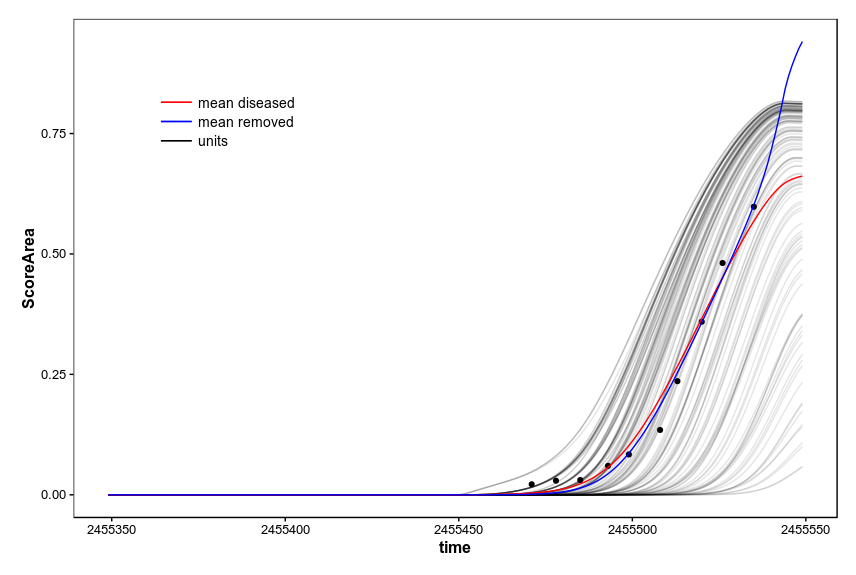
\includegraphics[width=0.6\textwidth]{figures/archidemio_cinetique}
\end{center}
$\Rightarrow$ Utiliser les connaissances sur les méthodes pour calibrer le modèle sur l'ensemble des paramètres

\end{frame}

\end{document}



%%%Local Variables:
%%% mode: latex
%%% eval: (TeX-PDF-mode 1)
%%% ispell-local-dictionary: "francais"
%%% eval: (flyspell-mode 1)
%%%End:


